\documentclass[12pt]{article}

\usepackage[english]{babel}
\usepackage[utf8]{inputenc}
\usepackage{sansmathfonts}
\usepackage[T1]{fontenc}
\renewcommand*\familydefault{\sfdefault} %% Only if the base font of the document is to be sans serif
\usepackage{multicol,lipsum}
\usepackage{amsmath,cancel}
\usepackage{amssymb,amsthm,dsfont,mathrsfs}
\usepackage[colorinlistoftodos]{todonotes}
\usepackage{geometry}
\geometry{
a4paper,
total={170mm,257mm},
left=20mm,
top=15mm,
bottom=22mm,
}
\usepackage{natbib}
\usepackage{soul}
\usepackage{setspace}
\usepackage{hyperref}
\usepackage{xcolor}
\usepackage{graphicx}
\usepackage{tikz}
\usepackage{siunitx}
\graphicspath{ {imagens/} }
\usepackage{fancyhdr}
\pagestyle{fancy}
\renewcommand{\headrulewidth}{0pt}

\color{darkgray}
\newcommand{\T}[1]{\vspace{0.4cm}\textbf{\large#1}}
\newcommand{\TW}[1]{\textbf{\large#1}}

\newcommand{\TM}[1]{\vspace{0.2cm} \textbf{#1}}

\newcommand{\M}[1]{
\vspace{-0.6cm}
\begin{flalign*}
#1&
\end{flalign*}
\vspace{-0.6cm}
}


\definecolor{bluebell}{rgb}{0.25, 0.35, 0.89} 
\definecolor{laranja}{rgb}{0.87, 0.48, 0.25} 
\definecolor{verde}{rgb}{0, 0.54, 0.44} 
\definecolor{babypink}{rgb}{1, 0.42, 0.52} 
\definecolor{rosa}{rgb}{1, 0.72, 0.77} 
\definecolor{cinza}{rgb}{0.3, 0.3, 0.3}  
\definecolor{iris}{rgb}{0.25, 0.35, 0.89}  
\definecolor{babyblue}{rgb}{0.13, 0.59, 0.95}

\setlength\columnsep{30pt}

\setlength{\parindent}{0cm}
\setlength{\fboxrule}{1.3pt}  % <-- Aumenta a espessura

\newcommand{\Formula}[1]{
\begin{center}
\color{iris}
\fcolorbox{rosa}{white}{
\(
\begin{array}{c}
#1
\end{array}
\)
}
\color{cinza}
\end{center}
}

\begin{document}
\pagenumbering{gobble}
\setstretch{1.3}


\includegraphics[width=4cm]{Logo2.png}
\begin{center}
    \textbf{\Huge \textcolor{bluebell}{Conjuntos}}
\end{center}

\begin{multicols}{2}

\T{Definição}

Um conjunto é uma coleção bem definida de elementos (objetos, números, pessoas etc.). Os elementos de um conjunto devem ser distintos e claramente identificáveis.

\T{Formas de representação}

Existem algumas formas comuns de representar um conjunto. A seguir apresentamos as principais formas.

\TM{Listagem ou Enumeração}

A Listagem ou Enumeração consiste em listar todos os elementos entre chaves.

\hspace{1cm}Exemplo: $A = \{1, 2, 3, 4, 5\}$. 

\TM{Propriedade Característica}

Outra forma de representação é por característica. Nesta abordagem os elementos são descritos por uma propriedade que eles possuem em comum. 

\hspace{1cm}Exemplo: $B = \{x | x \text{ é um número par}\}$. Este conjunto representa todos os números pares. Lemos "$x$ tal que $x$ é um número par".

\TM{Diagramas de Venn}

Representações gráficas que facilitam o entendimento das relações entre conjuntos, usando círculos dentro de um retângulo (o universo).

\TM{Exemplo}

\begin{center}
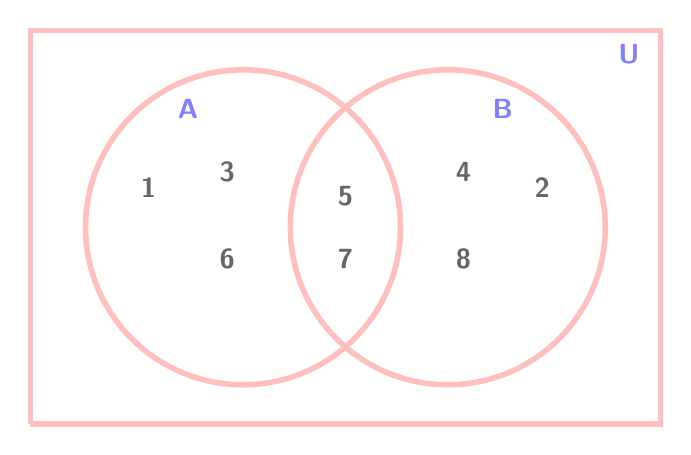
\begin{tikzpicture}
\tikzstyle{texto}=[draw=none,fill=none,black!60!white]
\tikzstyle{line}=[pink,line width=2pt]
\tikzstyle{line2}=[blue!50!white,line width=3pt]
\tikzstyle{angleA}=[draw=none,fill=blue!50!white]
\tikzstyle{angleB}=[draw=none,fill=blue!30!white]

\node[line2] at (-2,1.5) {\textbf{A}};
\node[line2] at (2,1.5) {\textbf{B}};
\node[line2] at (3.6,2.2) {\textbf{U}};

\node[texto] at (-2.5,0.5) {\textbf{1}};
\node[texto] at (-1.5,0.7) {\textbf{3}};
\node[texto] at (-1.5,-0.4) {\textbf{6}};

\node[texto] at (2.5,0.5) {\textbf{2}};
\node[texto] at (1.5,0.7) {\textbf{4}};
\node[texto] at (1.5,-0.4) {\textbf{8}};

\node[texto] at (0,0.4) {\textbf{5}};
\node[texto] at (0,-0.4) {\textbf{7}};

\draw[line] (-4,-2.5) -- (-4,2.5) -- (4,2.5) -- (4,-2.5) -- (-4,-2.5);

\draw[line] (-1.3,0) circle (2);
\draw[line] (1.3,0) circle (2);

\end{tikzpicture}
\end{center}

Nesse exemplo temos o conjunto $A=\{1, 3, 5, 6, 7\}$ e $B=\{2, 4, 5, 7, 8\}$ sendo representados pelo diagrama de Venn.

\T{Cardinalidade}

A cardinalidade de um conjunto é a medida do tamanho do conjunto, ou seja, o número de elementos distintos que ele contém. A principal notação para representar a cardinalidade de um conjunto $A$ é $|A|$.

\TM{Exemplo}

Se o conjunto $A = \{2, 6, 9\}$, então a cardinalidade de $A$ é $3$, e representamos como $|A| = 3$.

\T{Pertinência $(\in)$}

Indica que um elemento pertence a um conjunto. Ou seja, $x \in A$, indica que o elemento $x$ pertence ao conjunto $A$. Para indicar que um elemento não pertence ao conjunto utilize $x \notin A$.

\TM{Exemplos}

Dado o conjunto $A = \{3, 6, 7, 11\}$ temos que:

$3 \in A$ (3 pertence ao conjunto A).

$4 \notin A$ (4 não pertence ao conjunto A).

\T{Tipos Especiais de conjuntos}

Conjunto Vazio ($\emptyset$ ou $\{\}$): É o conjunto que não possui nenhum elemento.

\hspace{1cm}Exemplo: O conjunto de todos os números pares que são ímpares é o conjunto vazio.
 
Conjunto Unitário: Um conjunto com apenas um elemento.

\hspace{1cm}Exemplo: $\{5\}$.
     
Conjunto Universo ($U$): Em um dado contexto, é o conjunto que contém todos os elementos considerados.
 
Conjunto Finito: Possui um número limitado de elementos.
 
Conjunto Infinito: Possui um número ilimitado de elementos.

\hspace{1cm}Exemplo: O conjunto dos números naturais ($\mathbb{N} = \{1, 2, 3, ...\}$).

\T{União ($\cup$)}

A operação de união de conjuntos representa o conjunto de todos os elementos que pertencem a pelo menos um dos conjuntos.

\TM{Exemplo}

Se $A = \{1, 2, 3\}$ e $B = \{3, 4, 5\}$, então $A \cup B = \{1, 2, 3, 4, 5\}$.

\T{Interseção ($\cap$)}

Essa operação representa o conjunto de todos os elementos que pertencem a ambos os conjuntos.

\TM{Exemplo}

Se $A = \{1, 2, 3\}$ e $B = \{3, 4, 5\}$, então $A \cap B = \{3\}$.

\T{Diferença ($-$ ou $\setminus$)}

O conjunto de todos os elementos que pertencem ao primeiro conjunto, mas não pertencem ao segundo.

\TM{Exemplo}

Se $A = \{1, 2, 3\}$ e $B = \{3, 4, 5\}$, então $A - B = \{1, 2\}$.

\T{Complementar ($A^c$ ou $\bar{A}$ ou $A'$)}
 
Em relação a um conjunto universo $U$, o complementar de $A$ é o conjunto de todos os elementos de $U$ que não estão em $A$.

\TM{Exemplo}

Se $U = \{1, 2, 3, 4, 5\}$ e $A = \{1, 2\}$, então $A^c = \{3, 4, 5\}$.

\T{Fórmula da Diferença de Conjuntos}

\Formula{|A - B| = |A| - |A \cap B|}

Essa fórmula é utilizada para calcular o número de elementos do conjunto diferença entre A e B. 
Ou seja, a cardinalidade de $A - B$ é a cardinalidade de $A$ menos o número de elementos da intersecção entre $A$ e $B$. 

\TM{Exemplo}

$A = \{1, 2, 3, 4, 5\}, \quad |A| = 5$

$B = \{4, 5, 6, 7\}, \quad |B| = 4$

$A \cap B = \{4, 5\}, \quad |A \cap B| = 2$ 

Agora, aplicando a fórmula:

$|A - B| = |A| - |A \cap B|$

$|A - B| = 5 - 2 = 3$

Deste modo, sabemos que o número de elementos que estão no conjunto a e não estão no conjunto B é 3. 

\T{Fórmula da União de Conjuntos}

\Formula{|A \cup B| = |A| + |B| - |A \cap B|}

Essa fórmula é uma das mais fundamentais na teoria dos conjuntos e na combinatória, utilizada para calcular o número de elementos (ou cardinalidade) da união de dois conjuntos, $A$ e $B$.

\TM{Exemplo}

$A = \{1, 2, 3, 4\}, \quad |A| = 4$

$B = \{3, 4, 5, 6\}, \quad |B| = 4$ 

$A \cap B = \{3, 4\}, \quad |A \cap B| = 2$ 

Agora, aplicando a fórmula:

$|A \cup B| = |A| + |B| - |A \cap B|$

$|A \cup B| = 4 + 4 - 2 = 6$

Essa fórmula é uma ferramenta essencial para calcular o número de elementos na união de dois conjuntos, garantindo que elementos compartilhados não sejam contados em duplicidade.

\TM{Outra versão}

Usando a formula da subtração de dois conjuntos podemos elaborar uma outra versão da formula da união de dois conjuntos que pode facilitar na resolução de alguns problemas.

\Formula{|A \cup B| = |A-B| + |B-A| + |A \cap B|}

Nesta fórmula temos que a união dos conjuntos $A$ e $B$ é presentada pela soma do número de elementos exclusivos de $A$ mais os elementos exclusivos de $B$ mais os elementos da intersecção de $A \cap B$.

A seguir apresentamos o diagrama de Venn apresentando a cardinalidade das principais partes dos conjuntos.

\begin{center}
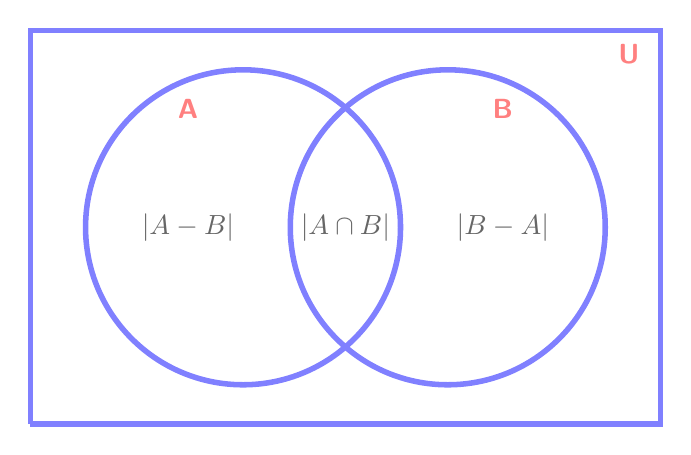
\begin{tikzpicture}
\tikzstyle{texto}=[draw=none,fill=none,black!60!white]
\tikzstyle{line}=[blue!50!white,line width=2pt]
\tikzstyle{line2}=[red!50!white,line width=3pt]
\tikzstyle{angleA}=[draw=none,fill=blue!50!white]
\tikzstyle{angleB}=[draw=none,fill=blue!30!white]

\node[line2] at (-2,1.5) {\textbf{A}};
\node[line2] at (2,1.5) {\textbf{B}};
\node[line2] at (3.6,2.2) {\textbf{U}};

\node[texto] at (-2,0) {\textbf{$|A-B|$}};

\node[texto] at (2,0) {\textbf{$|B-A|$}};

\node[texto] at (0,0) {\textbf{$|A \cap B|$}};

\draw[line] (-4,-2.5) -- (-4,2.5) -- (4,2.5) -- (4,-2.5) -- (-4,-2.5);

\draw[line] (-1.3,0) circle (2);
\draw[line] (1.3,0) circle (2);

\end{tikzpicture}
\end{center}


\TM{Exemplo}

$A = \{2, 4, 5, 7\}, \quad |A| = 4$

$B = \{2, 4, 8\}, \quad |B| = 3$ 

$A-B = \{5, 7\}, \quad |A-B| = 2$ 

$B-A = \{8\}, \quad |B-A| = 1$ 

$A \cap B = \{2, 4\}, \quad |A \cap B| = 2$ 

Agora, aplicando a fórmula:

$|A \cup B| = |A-B| + |B-A| + |A \cap B|$

$|A \cup B| = 2 + 1 + 2 = 5$

\begin{center}
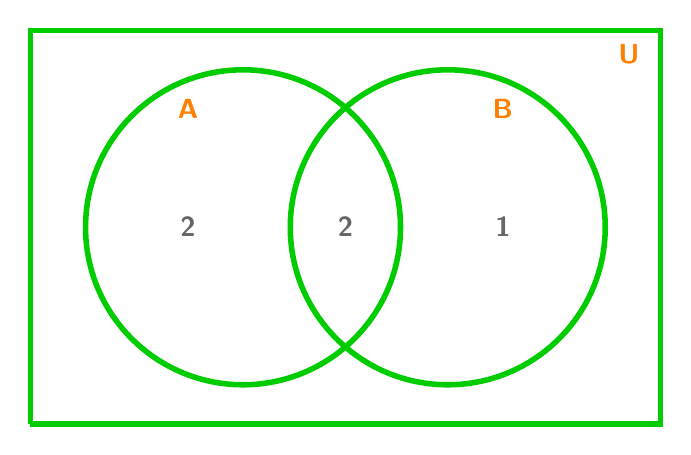
\begin{tikzpicture}
\tikzstyle{texto}=[draw=none,fill=none,black!60!white]
\tikzstyle{line}=[green!80!black,line width=2pt]
\tikzstyle{line2}=[orange,line width=3pt]
\tikzstyle{angleA}=[draw=none,fill=blue!50!white]
\tikzstyle{angleB}=[draw=none,fill=blue!30!white]

\node[line2] at (-2,1.5) {\textbf{A}};
\node[line2] at (2,1.5) {\textbf{B}};
\node[line2] at (3.6,2.2) {\textbf{U}};

\node[texto] at (-2,0) {\textbf{2}};

\node[texto] at (2,0) {\textbf{1}};

\node[texto] at (0,0) {\textbf{2}};

\draw[line] (-4,-2.5) -- (-4,2.5) -- (4,2.5) -- (4,-2.5) -- (-4,-2.5);

\draw[line] (-1.3,0) circle (2);
\draw[line] (1.3,0) circle (2);

\end{tikzpicture}
\end{center}



As noções de conjunto são a base para muitos outros conceitos na matemática, como funções, relações, probabilidade e lógica. Compreender esses fundamentos é crucial para o estudo avançado de diversas áreas da matemática e outras ciências.

\end{multicols}
\lfoot{\scriptsize © Copyright, Pratique Já}
\cfoot{\large \textcolor{bluebell}{pratiqueja.com}}
\end{document}